\documentclass[conference]{IEEEtran}
\usepackage{graphicx} % Required for inserting images
\usepackage{booktabs}
\usepackage{url}

% Suggested title; replace if preferred.
\title{Can One Recurrent Spiking Layer Replace Dedicated Spatial and Temporal Filters for Cross-Session Motor Imagery EEG Decoding?}
\author{\IEEEauthorblockN{[Author 1], [Author 2], [Author 3]}
\IEEEauthorblockA{[Affiliation]}}
\date{November 2026}

\begin{document}

\maketitle

\begin{abstract}
Brain--computer interfaces (BCIs) that decode motor imagery from the electroencephalogram (EEG) could help people with complex mobility needs control assistive devices, but low decoding accuracy limits their use. Motor imagery information is both spatial and temporal, and EEGNet extracts it with separate temporal, spatial and feature-summarizing layers. This paper tested whether a single layer of a recurrent spiking neural network (RSNN), whose neurons are connected through trained recurrent weights and receive the EEG one sample at a time, can replace these three layers. A 17-neuron RSNN matched to EEGNet's parameter count and a 2560-neuron RSNN matched to its number of hidden units were compared with EEGNet, a spiking conversion of EEGNet and a non-spiking recurrent network, which separate the effects of spiking and recurrence. On BCI Competition IV dataset 2a (nine able-bodied adults), each model was pretrained on other subjects, fine-tuned on the target subject's first session and tested on the second. Mean session-2 accuracy was 0.600 for EEGNet, 0.565 for the converted SNN, 0.411 for the recurrent network, and 0.385 and 0.341 for the two RSNNs. The 17-neuron RSNN was less accurate than EEGNet in all nine subjects (median paired difference $-0.222$, Holm-corrected $p = 0.020$) but exceeded chance in six. The effect of spiking was small and not significant in either architecture, so most of the deficit came from replacing EEGNet's dedicated layers with one recurrent layer. The small sample and the use of hyperparameters chosen for EEGNet limit this conclusion.
\end{abstract}

\begin{IEEEkeywords}
Brain--computer interface, motor imagery, EEG, spiking neural network, recurrent spiking neural network, EEGNet, spatio-temporal feature extraction
\end{IEEEkeywords}

\section{Introduction}
\label{sec:intro}

A brain--computer interface (BCI) translates measured brain activity into commands for an external device. For people with complex mobility needs, a BCI that decodes the electroencephalogram (EEG) could provide direct control of a wheelchair or other mobility device without relying on residual movement \cite{padfield2019}. Motor imagery is a common control signal for such systems. Imagining a movement of the left hand, right hand, feet or tongue changes the power of the mu (8--13~Hz) and beta (13--30~Hz) rhythms over the sensorimotor cortex, and these changes can be detected in the scalp EEG \cite{mcfarland2000,pfurtscheller2006}.

Low decoding accuracy remains one of the main barriers to reliable use of motor imagery BCIs \cite{padfield2019}. EEG has a low signal-to-noise ratio, changes within and between recording sessions, differs between people and is usually recorded in small datasets \cite{padfield2019}. A decoder for a new user must also cope with a later session whose signals differ from those recorded during calibration.

Neural networks have become a standard approach to this problem because they learn features directly from the signal instead of relying on hand-designed filters. Motor imagery information is both spatial and temporal. The band-power changes are distributed over particular electrodes and are carried by oscillations that develop over the trial. EEGNet is a compact convolutional neural network (CNN) that extracts these in three dedicated layers \cite{lawhern2018}. A temporal convolution learns frequency filters, a depthwise convolution learns spatial filters across electrodes, and a separable convolution summarizes the resulting feature maps over time before a dense layer classifies the trial. The configuration used on this dataset has 796 trainable parameters. Each convolution sees a window of many samples at once, so the network does not need to hold earlier input in memory.

Spiking neural networks (SNNs) process information differently. Instead of passing continuous activations between layers, each neuron integrates its input in a membrane potential and emits a discrete event, a spike, when that potential crosses a threshold. This representation is closer to the way biological neurons communicate than the continuous units of a conventional artificial neural network (ANN) \cite{maass1997}, and the event-driven computation has made SNNs a candidate for low-power embedded and neuromorphic hardware \cite{liao2025,zhang2025}. SNNs have already been applied to motor imagery decoding, including on BCI Competition IV dataset 2a \cite{liao2025,chen2026,zhang2025}, and an SNN converted from EEGNet performed comparably to the original \cite{chen2026}. SNNs have generally been somewhat less accurate than comparable CNNs \cite{zhang2025}.

Most SNNs used for motor imagery are feedforward \cite{liao2025,chen2026}. Information passes from one layer to the next, and in a converted EEGNet the temporal features come from the convolutions. A neuron in such a network can carry information forward in time only through its own state, which this paper calls \emph{intra-recurrence}: its membrane potential and, in a recurrent layer, its trained connection to itself. In a leaky integrate-and-fire (LIF) neuron the membrane potential decays gradually, so earlier input continues to influence the neuron for a short time. A feedforward SNN has no \emph{inter-recurrence}, meaning no trained connections between different neurons of the same layer that feed activity back into the population. A recurrent spiking neural network (RSNN) adds these connections. They form loops, so activity in one neuron at one time step drives other neurons at the next, and a pattern of activity can circulate through the population. Because its state carries information forward, an RSNN can in principle receive the EEG one sample at a time and extract spatial and temporal features in a single layer. Its input weights combine the electrodes at each step, and its recurrence integrates the result over time. This paper asks whether one such recurrent layer can do the work of EEGNet's dedicated temporal, spatial and feature-summarizing layers.

The motivation for considering RSNNs for EEG decoding is also biological. EEG reflects the summed activity of large cortical populations \cite{buzsaki2012}, which are densely and recurrently connected \cite{douglas2007}, and recurrent excitation in such circuits is thought to sustain the persistent activity that underlies short-term memory \cite{wang2001}. A decoder that combines spiking neurons with trained recurrent connections is therefore a more biologically plausible model of the processes that generate the signal. Whether this plausibility leads to more accurate decoding is a hypothesis, not an established result. RSNNs have performed well on other temporal signals. Recurrent networks of adaptive spiking neurons reached state-of-the-art SNN accuracy on speech and gesture benchmarks at publication \cite{yin2021}, and recurrent SNNs outperformed feedforward SNNs in decoding motor cortex spike trains \cite{liu2025,liu2024}. Those inputs, however, are already sequences of spikes, whereas EEG is a continuous scalp signal that must first be converted into an input current.

Recurrence itself is not new to motor imagery decoding. Non-spiking networks of long short-term memory (LSTM) units and gated recurrent units (GRUs) \cite{hochreiter1997,cho2014} have been used to classify motor imagery EEG \cite{luo2018}, and recurrent elements have been added to spiking decoders, as spiking LSTM units \cite{gong2023} or as a recurrent network applied to spike-encoded EEG \cite{lim2025}. To the best of our knowledge, however, an RSNN, in which spiking neurons are connected to one another through trained inter-recurrent weights, has not been used to make motor imagery decoding more accurate, nor compared with EEGNet on a held-out recording session with subject-level statistics.

Going directly from EEGNet to an RSNN changes two things at once. The neurons become spiking, and EEGNet's dedicated layers are replaced by one recurrent layer. A difference in accuracy could come from either change, so this study compares five models. EEGNet (the ANN) is the reference model. An SNN converted from the trained EEGNet keeps EEGNet's layers and weights and changes only the neurons, so the ANN and SNN show the effect of spiking in the feedforward design. A non-spiking recurrent neural network (RNN-p) has the same single recurrent layer as the RSNNs but uses conventional exponential linear units (ELUs). The ANN and RNN-p therefore show the effect of replacing EEGNet's layers with recurrence without spiking, and RNN-p and RSNN-p show the effect of spiking within the recurrent layer. Two RSNNs were tested. RSNN-p has 17 recurrent neurons, chosen so that its parameter count (752) is close to those of EEGNet (796) and the converted SNN (776). RSNN-n has 2560 neurons, as many as EEGNet has hidden units, to test whether RSNN-p was limited by its small size. Each recurrent model receives one EEG sample (22 channel values) per time step and projects it linearly onto a single layer in which every neuron is connected to every other neuron and to itself. Its spatial extraction is therefore limited to this one projection, and its temporal extraction depends on recurrence. The trial is classified from the time-averaged activity of the layer. All weights of the RSNNs, including the recurrent ones, are trained with surrogate gradients \cite{neftci2019}.

The research question is whether RSNNs, which must extract spatial and temporal features within a single recurrent layer, can decode four-class motor imagery EEG from BCI Competition IV dataset 2a as accurately as EEGNet, which extracts them in dedicated layers, when each subject is tested on a separate, later recording session. The contribution is a subject-level, cross-session evaluation of two RSNNs against EEGNet, with spiking and non-spiking controls that separate the effects of spiking and recurrence, chance-level testing for every subject and paired statistics across subjects.

\section{Dataset and Methods}
\label{sec:methods}

\subsection{Dataset}

This study used BCI Competition IV Dataset 2a \cite{brunner2008,tangermann2012}, accessed through MOABB \cite{jayaram2018} (dataset BNCI2014\_001 \cite{moabbdoc2014001}) on October 8, 2026. Nine subjects (S1--S9) each completed two sessions on different days. In each trial an arrow cue at $t = 2$~s asked the subject to imagine moving the left hand, right hand, both feet or tongue until $t = 6$~s, without feedback. Each session has 288 trials (72 per class), giving 5{,}184 trials in total. EEG was recorded from 22 electrodes at 250~Hz. The three EOG channels were not used, as the dataset description requires \cite{brunner2008}. The input to every model is the EEG of one trial and the outcome is its class label, with a nominal chance accuracy of 25\%.

Trials from one subject share electrode placement, physiology and recording conditions, so the subject, not the trial, is the independent case, and all results are summarized per subject (Section~\ref{sec:eval}). No subject or trial was excluded. Trials marked by the dataset's expert as containing artifacts were kept, leaving 72 trials per class in every session. Fig.~\ref{fig:topo} shows the class-specific band-power changes in the preprocessed data.

\begin{figure}[!t]
  \centering
  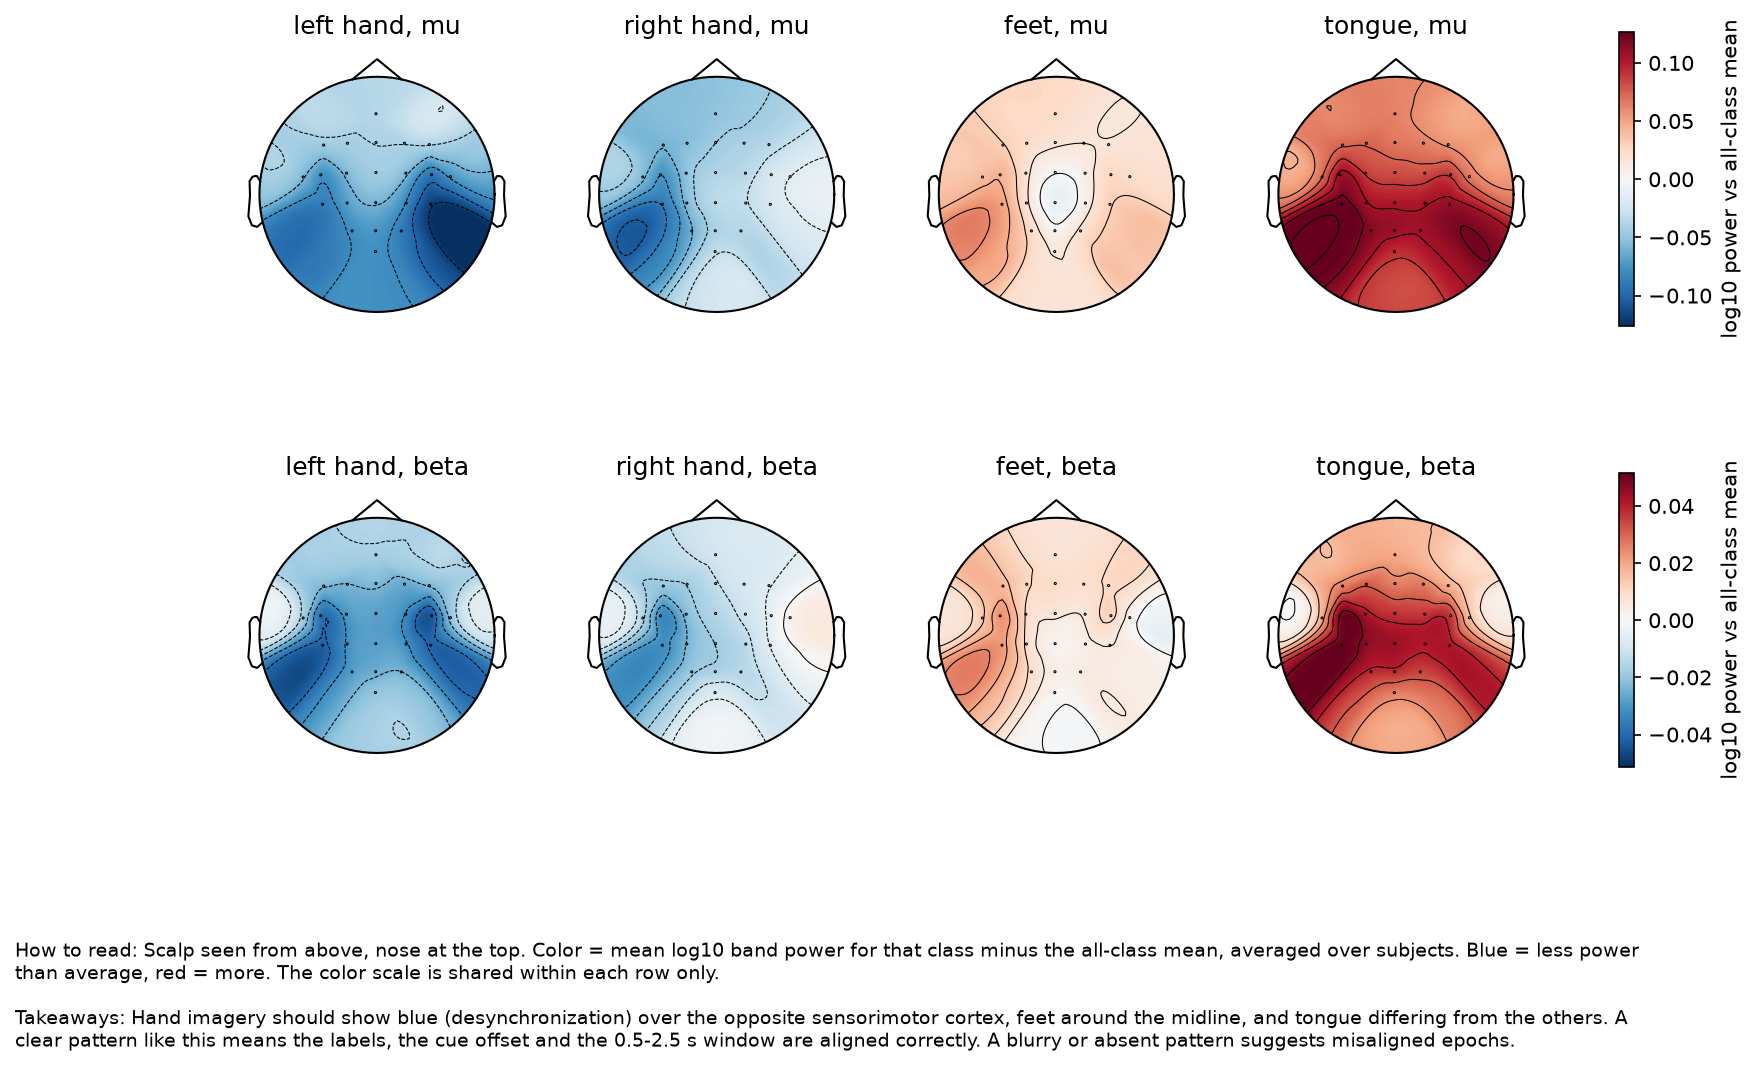
\includegraphics[width=\columnwidth, trim=0 133.4bp 0 0, clip]{figures/class_topomaps.png}
  \caption{Class-specific band power of the preprocessed data (all subjects, both sessions). Mean $\log_{10}$ mu (8--13~Hz, top) and beta (13--30~Hz, bottom) power of each class minus the mean over all classes, averaged over subjects. Blue indicates lower power than average.}
  \label{fig:topo}
\end{figure}

The competition review states that the data are freely available provided the review is cited \cite{tangermann2012}, and the competition website asks users to credit the group that recorded the data \cite{bciciv_web}, which is done here by citing \cite{brunner2008,naeem2006}. MOABB distributes the dataset under a CC BY-ND 4.0 license \cite{moabbdoc2014001}, so the recordings are not redistributed with this work. Subjects are identified only by code. No attempt was made to link them to other sources, and results are reported only by code or in aggregate. MOABB describes the subjects as healthy \cite{moabbdoc2014001}, and no age, sex or handedness is reported. Nine able-bodied subjects from one laboratory, recorded offline with a cue-based paradigm, are a small and narrow sample that does not include people with the motor impairments a BCI is meant to serve.

\subsection{Preprocessing and protocol}

The data providers had band-pass filtered the recordings at 0.5--100~Hz and applied a 50~Hz notch filter \cite{brunner2008}. Following EEGNet \cite{lawhern2018}, each run was further band-pass filtered at 4--40~Hz, resampled to 128~Hz and cut into epochs from 0.5 to 2.5~s after the cue, giving a $22 \times 256$ (channels $\times$ samples) input per trial. No artifact removal or baseline correction was applied.

Pretraining followed the cross-subject protocol of EEGNet \cite{lawhern2018}. For each target subject, the target was left out of pretraining entirely. Session~1 of five randomly chosen other subjects was used for pretraining (1{,}440 trials) and session~1 of the remaining three for pretraining validation (864 trials). Unlike in EEGNet, the model was then fine-tuned on the target's session~1 (230 training and 58 validation trials, stratified by class) and tested on its 288 session-2 trials, which were never used for training, model selection, input normalization or SNN calibration. This mimics a new user who records one calibration session and uses the BCI on a later day. The random split was repeated ten times per subject, giving 90 folds shared by all models.

\subsection{Models}

Fig.~\ref{fig:arch} shows the architectures and Table~\ref{tab:models} summarizes the five models.

\begin{figure*}[!t]
  \centering
  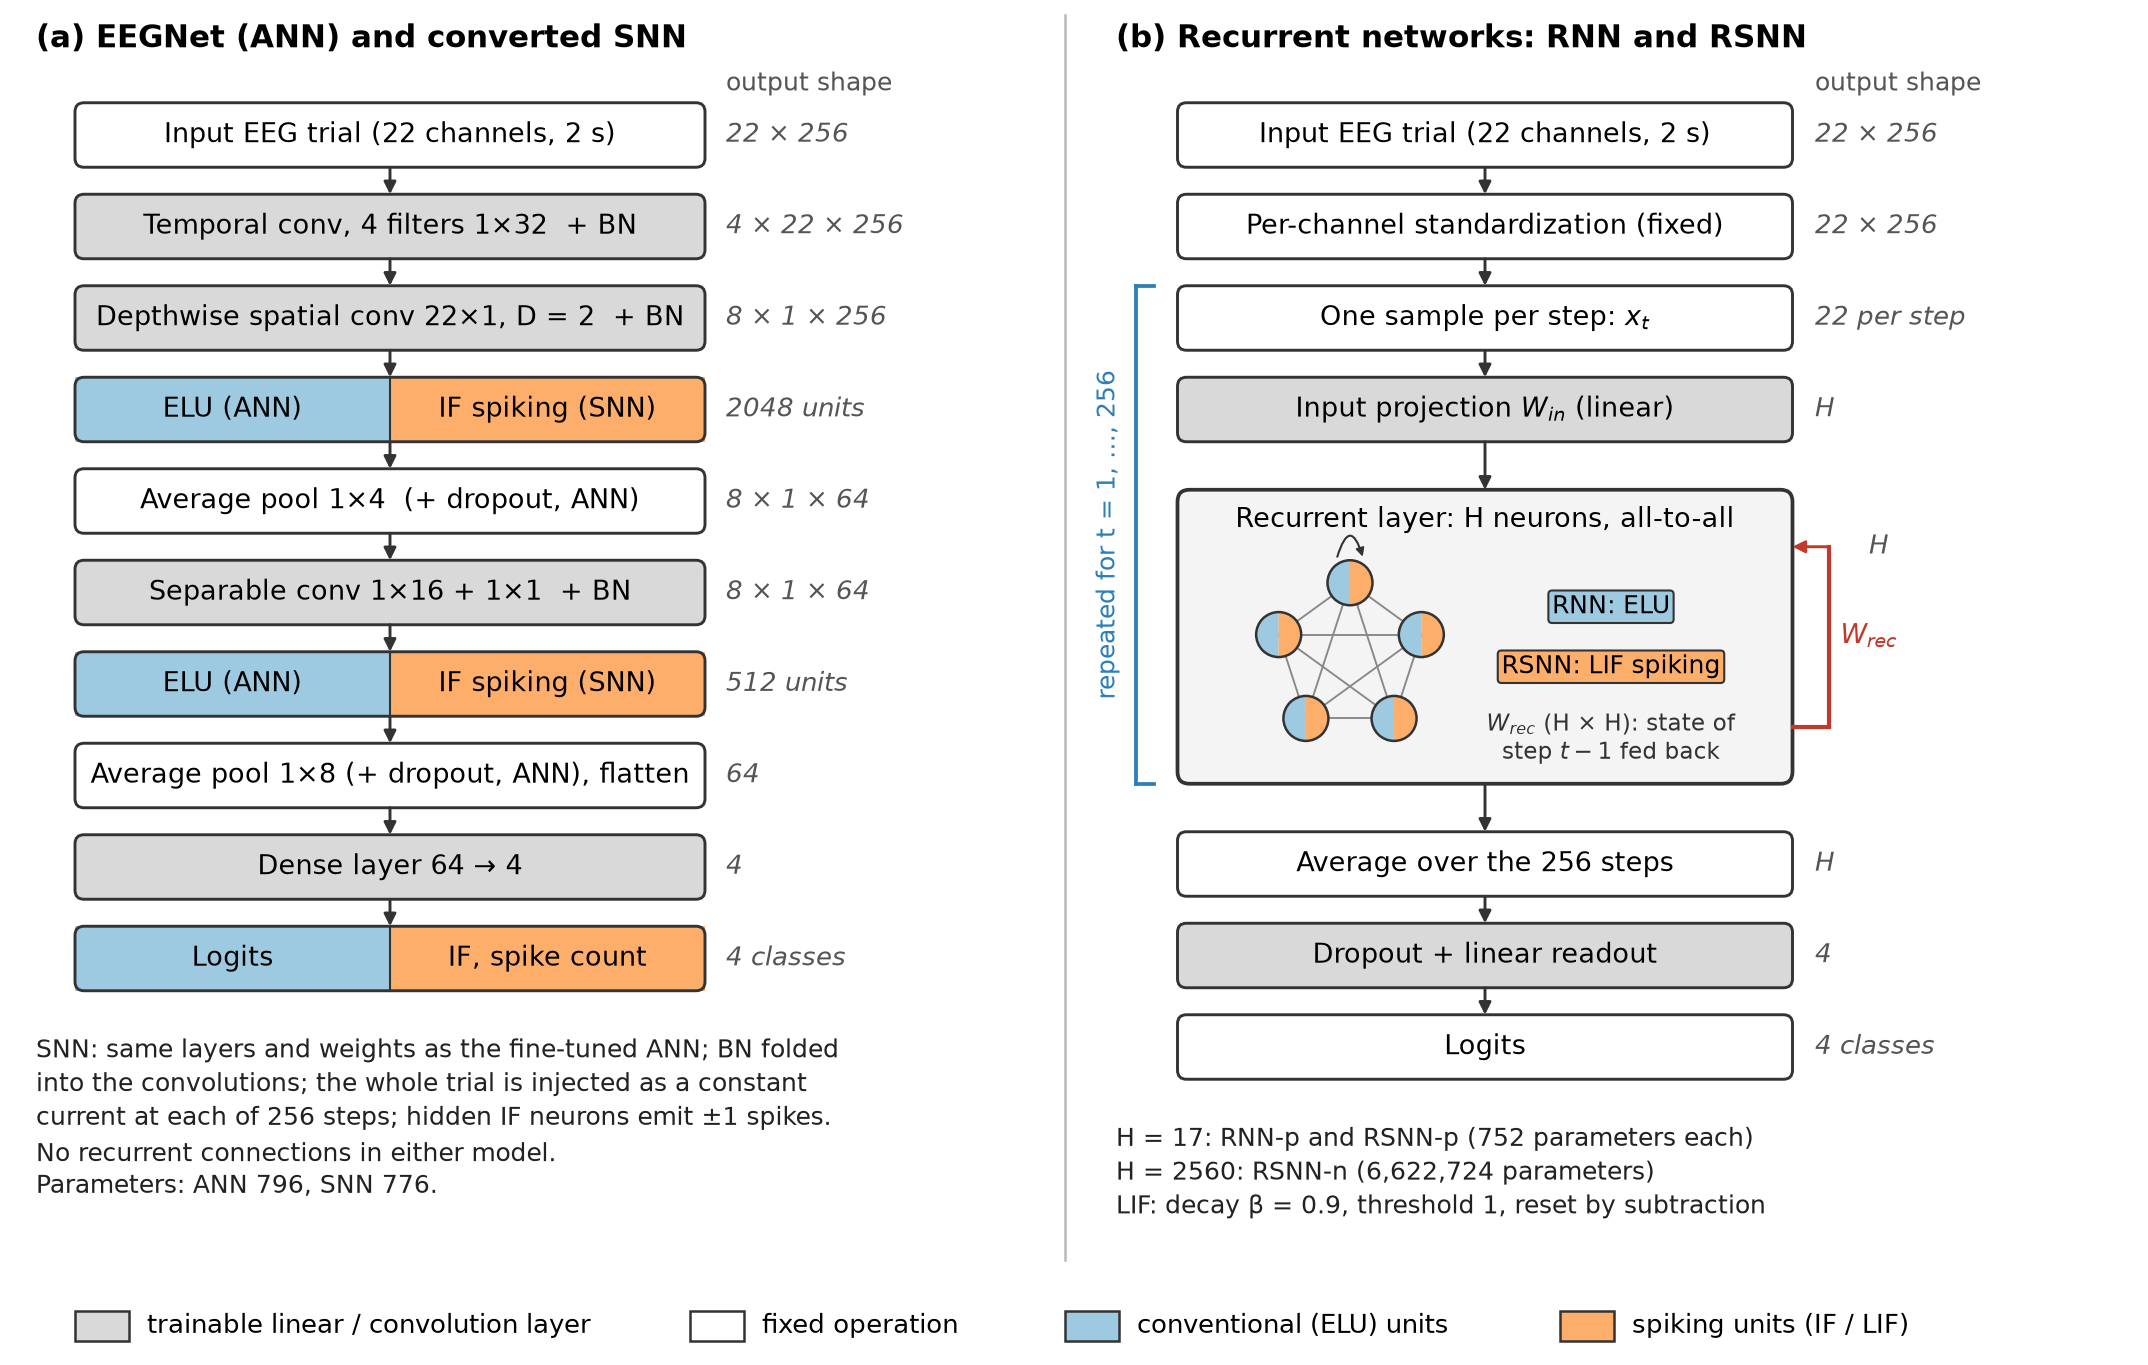
\includegraphics[width=\textwidth]{figures/model_architectures.png}
  \caption{Architectures of the implemented models. (a) EEGNet (ANN) and the SNN converted from it, which share layers and weights and differ only in their neurons. (b) The recurrent networks, which receive one EEG sample per step and feed every hidden neuron's state back to all hidden neurons through $W_{rec}$. The RNN uses ELU units and the RSNN leaky integrate-and-fire (LIF) spiking neurons. Shapes exclude the batch dimension.}
  \label{fig:arch}
\end{figure*}

\begin{table}[!t]
  \centering
  \caption{Compared models}
  \label{tab:models}
  \setlength{\tabcolsep}{4pt}
  \begin{tabular}{lcccr}
    \toprule
    Model & Neuron model & Recurrent & Hidden units & Parameters \\
    \midrule
    ANN (EEGNet) & ELU & No & 2560 & 796 \\
    SNN (converted) & IF, spiking & No & 2560 & 776 \\
    RNN-p & ELU & Yes & 17 & 752 \\
    RSNN-p & LIF, spiking & Yes & 17 & 752 \\
    RSNN-n & LIF, spiking & Yes & 2560 & 6{,}622{,}724 \\
    \bottomrule
  \end{tabular}
\end{table}

\textbf{ANN.} The baseline is EEGNet-4,2 \cite{lawhern2018}. A temporal convolution learns frequency filters, a depthwise convolution learns spatial filters across the 22 channels, a separable convolution summarizes the resulting feature maps over time, and a dense layer gives four class scores.

\textbf{SNN.} The feedforward SNN is each fold's fine-tuned ANN converted to a spiking neural network without retraining \cite{rueckauer2017}. It keeps the ANN's layers and weights, replaces each ELU with integrate-and-fire neurons that emit positive or negative spikes (Fig.~\ref{fig:arch}), and rescales the weights using the ANN's activations on the target's fine-tuning trials. The whole trial is applied as a constant input over 256 simulation steps, and the class whose output neurons fire most is the prediction.

\textbf{RNN.} The recurrent network has one layer of $H$ ELU units in which every unit is connected to every other unit and to itself. Its input is standardized per channel with statistics from the pretraining subjects only. It receives one EEG sample (22 values) per step, so 256 steps cover the trial. At each step every unit combines the current sample with the previous activity of all units through trained recurrent weights. The activity averaged over the 256 steps feeds a linear readout.

\textbf{RSNN.} The RSNNs are identical to the RNN except that the ELU units are replaced by leaky integrate-and-fire spiking neurons, with the same threshold as the SNN. Each neuron's decaying membrane potential and trained self-connection provide intra-recurrence, and the trained connections between neurons provide inter-recurrence. The feedforward SNN, by contrast, has no connections within a layer and receives the whole trial as a constant input, so its temporal features come from its convolutions. The RSNNs were trained with surrogate gradients \cite{neftci2019}.

\textbf{Network size.} RNN-p and RSNN-p use $H = 17$, giving 752 parameters, the closest match to the ANN's 796 and the SNN's 776. RSNN-p versus the ANN therefore tests the research question at an approximately equal parameter count. The ANN versus the SNN and RNN-p versus RSNN-p isolate the effect of spiking, and RNN-p versus the ANN isolates the effect of replacing EEGNet's layers with one recurrent layer. The recurrent and convolutional models also differ in input encoding and normalization, so this last comparison tests the recurrent design as a whole. RSNN-n uses $H = 2560$, the number of hidden neurons in EEGNet, to test whether RSNN-p was simply too small, since 17 neurons may lack the capacity to represent the spatial and temporal patterns of four classes.

\subsection{Training}
\label{sec:training}

The ANN and the recurrent models were trained with one shared procedure that follows EEGNet where possible \cite{lawhern2018}. It used the Adam optimizer with default parameters (learning rate $10^{-3}$), cross-entropy loss and 500 pretraining epochs, and kept the weights with the lowest validation loss at the end of each phase. EEGNet used a dropout probability of 0.25 for cross-subject training and 0.5 for training on a single subject's smaller data set, so 0.25 was used for pretraining and 0.5 for fine-tuning. Fine-tuning, which EEGNet did not include, ran for 100 epochs. All models were trained in batches of 16 trials.

Gradients were clipped to a global L2 norm of 1.0. Whenever the norm of the full gradient vector exceeded 1.0, it was rescaled to that norm before the parameter update, which limits the size of each update without changing its direction. Recurrent networks trained by backpropagation through many time steps, here 256, are prone to exploding gradients \cite{bengio1994,pascanu2013}, and clipping the gradient norm was proposed as a remedy \cite{pascanu2013}. The threshold of 1.0 was not tuned. The same clipping was applied to every trained model so that the training procedure stayed identical across models. Using one set of settings keeps the comparison controlled and never uses test data for model selection. Tuning each model separately was out of scope. The SNN was not trained. The code was written in Python with PyTorch, run on the University of Calgary's ARC cluster, and is available at \url{https://github.com/thesixtium/bmen-600-group-11}. Exact hyperparameters, implementation details and software versions are given in the repository and are not repeated here.

\subsection{Evaluation}
\label{sec:eval}

Accuracy on session~2 is the primary measure, because low accuracy is one of the main barriers to practical motor imagery BCIs \cite{padfield2019}. With balanced classes it equals balanced accuracy. Cohen's $\kappa$ corrects for chance, and macro-averaged F1 falls if a model ignores a class. Confusion matrices pooled over subjects and repeats give per-class recall.

The ten repeats of each subject were averaged, giving nine paired values per model and metric, summarized as mean $\pm$ SD across subjects. A result was called above chance only if it exceeded the binomial threshold for 288 trials (29.2\%, $\alpha = 0.05$) \cite{combrisson2015} and a 10{,}000-shuffle label permutation test ($p < 0.05$). The binomial threshold is the accuracy that random guessing among four balanced classes would exceed with a probability of only 5\% on 288 test trials. It lies above the nominal 25\% because a finite test set lets random guessing reach accuracies above 25\% by chance. The permutation test builds the same reference empirically by shuffling the test labels against the model's predictions.

The primary comparisons were RSNN-p vs.\ ANN (the research question), RSNN-p vs.\ SNN, ANN vs.\ SNN (effect of spiking in the feedforward design), RNN-p vs.\ RSNN-p (effect of spiking in the recurrent design) and RNN-p vs.\ ANN (effect of recurrence without spiking). A secondary family compared RSNN-n with RSNN-p and the SNN. Each paired difference was tested with an exact two-sided Wilcoxon signed-rank test, with Holm correction within each family and metric, and reported as the median difference with a bootstrap 95\% confidence interval over subjects. With nine subjects the smallest possible $p$ is about 0.004 ($2/2^9$, reached when all nine differences have the same sign), so only effects consistent across nearly all subjects can reach significance, which guards against small random differences \cite{tangermann2012}. Because the Holm correction multiplies the smallest $p$ in a family by the number of comparisons, the smallest attainable corrected values are 0.020 in the primary family (five comparisons) and 0.012 in the secondary family.

Three secondary analyses support the interpretation. Each trained model's pretrained checkpoint was tested on session~2 without target data (zero-shot) to measure the gain from fine-tuning (Wilcoxon, Holm across the four trained models, for which the smallest attainable corrected $p$ is 0.016). Training and validation loss curves were summarized by their median over subjects. The loss is the cross-entropy, the negative logarithm of the probability that the model assigns to the correct class, averaged over trials. A model that cannot distinguish the classes and assigns a probability of 1/4 to each class has a loss of $-\ln(1/4) = \ln 4 \approx 1.386$, so $\ln 4$ is the chance-level loss in this four-class task, and a validation loss near $\ln 4$ means that nothing that generalizes has been learned. A loss spike was defined as an epoch in which the training or validation loss exceeded $10\ln 4 \approx 13.9$, which requires the model to be confidently wrong on most trials and therefore marks sudden training failures rather than ordinary over- or underfitting. Finally, agreement of subject rankings across models was measured with Kendall's $W$ (1 if all models rank the subjects identically, 0 if their rankings are unrelated) and a split of accuracy variance into subject, model and residual parts. Each subject's mean accuracy was also correlated (Spearman, uncorrected) with signal measures from the preprocessed EEG. These were class separability of mu and beta band power at C3, Cz and C4, between-session band-power and covariance shift, trial-amplitude variability and the rate of trials exceeding $\pm 100~\mu$V, a common amplitude criterion for artifacts \cite{zhangluck2025}.

\section{Results}

\subsection{Recurrent versus non-recurrent decoding}

The non-recurrent models outperformed the recurrent models in every subject (Fig.~\ref{fig:acc}). Mean session-2 accuracy was $0.600 \pm 0.150$ for the ANN, $0.565 \pm 0.154$ for the SNN, $0.411 \pm 0.106$ for RNN-p, $0.385 \pm 0.100$ for RSNN-p and $0.341 \pm 0.085$ for RSNN-n. Cohen's $\kappa$ (0.466, 0.421, 0.215, 0.180, 0.122) and macro F1 (0.586, 0.542, 0.378, 0.340, 0.294) gave the same order. The ANN and SNN exceeded chance in all nine subjects, RNN-p in seven, RSNN-p in six and RSNN-n in five.

Table~\ref{tab:paired} gives the paired comparisons that answer the research question. RSNN-p was less accurate than the ANN in all nine subjects (median paired difference $-0.222$, 95\% CI $[-0.304, -0.138]$, $p_\mathrm{Holm} = 0.020$) and less accurate than the SNN. Replacing EEGNet's layers with one non-spiking recurrent layer (RNN-p $-$ ANN) also lowered accuracy in all nine subjects. The two spiking comparisons, ANN $-$ SNN and RNN-p $-$ RSNN-p, were small and not significant, with the non-spiking model ahead in seven of nine subjects. Kappa and macro F1 led to the same conclusion for every comparison. On test trials that the ANN misclassified, RSNN-p and RNN-p were correct 26\% of the time, close to the 25\% expected from guessing.

\begin{table}[!t]
  \centering
  \caption{Paired differences in session-2 accuracy}
  \label{tab:paired}
  \setlength{\tabcolsep}{3pt}
  \resizebox{\columnwidth}{!}{%
  \begin{tabular}{llcccc}
    \toprule
    Comparison & Effect & Median & 95\% CI & $n$ & $p_\mathrm{Holm}$ \\
    \midrule
    RSNN-p $-$ ANN & Research question & $-0.222$ & $[-0.304, -0.138]$ & 9/9 & 0.020 \\
    RSNN-p $-$ SNN & Recurrent design & $-0.142$ & $[-0.264, -0.092]$ & 9/9 & 0.020 \\
    RNN-p $-$ ANN & Recurrence & $-0.196$ & $[-0.254, -0.130]$ & 9/9 & 0.020 \\
    ANN $-$ SNN & Spiking (FF) & $+0.047$ & $[-0.020, 0.081]$ & 7/9 & 0.148 \\
    RNN-p $-$ RSNN-p & Spiking (rec.) & $+0.031$ & $[-0.007, 0.063]$ & 7/9 & 0.148 \\
    \midrule
    RSNN-n $-$ RSNN-p & Size & $-0.041$ & $[-0.084, -0.013]$ & 9/9 & 0.012 \\
    RSNN-n $-$ SNN & Size & $-0.234$ & $[-0.315, -0.130]$ & 9/9 & 0.012 \\
    \bottomrule
  \end{tabular}}
  \\[2pt]
  \footnotesize Difference = first minus second model, median over subjects of each subject's mean over 10 repeats, with a bootstrap 95\% CI over subjects. $n$: subjects whose difference has the sign of the median. FF: feedforward; rec.: recurrent. Holm correction within the primary (top) and secondary (bottom) family.
\end{table}

\begin{figure*}[!t]
  \centering
  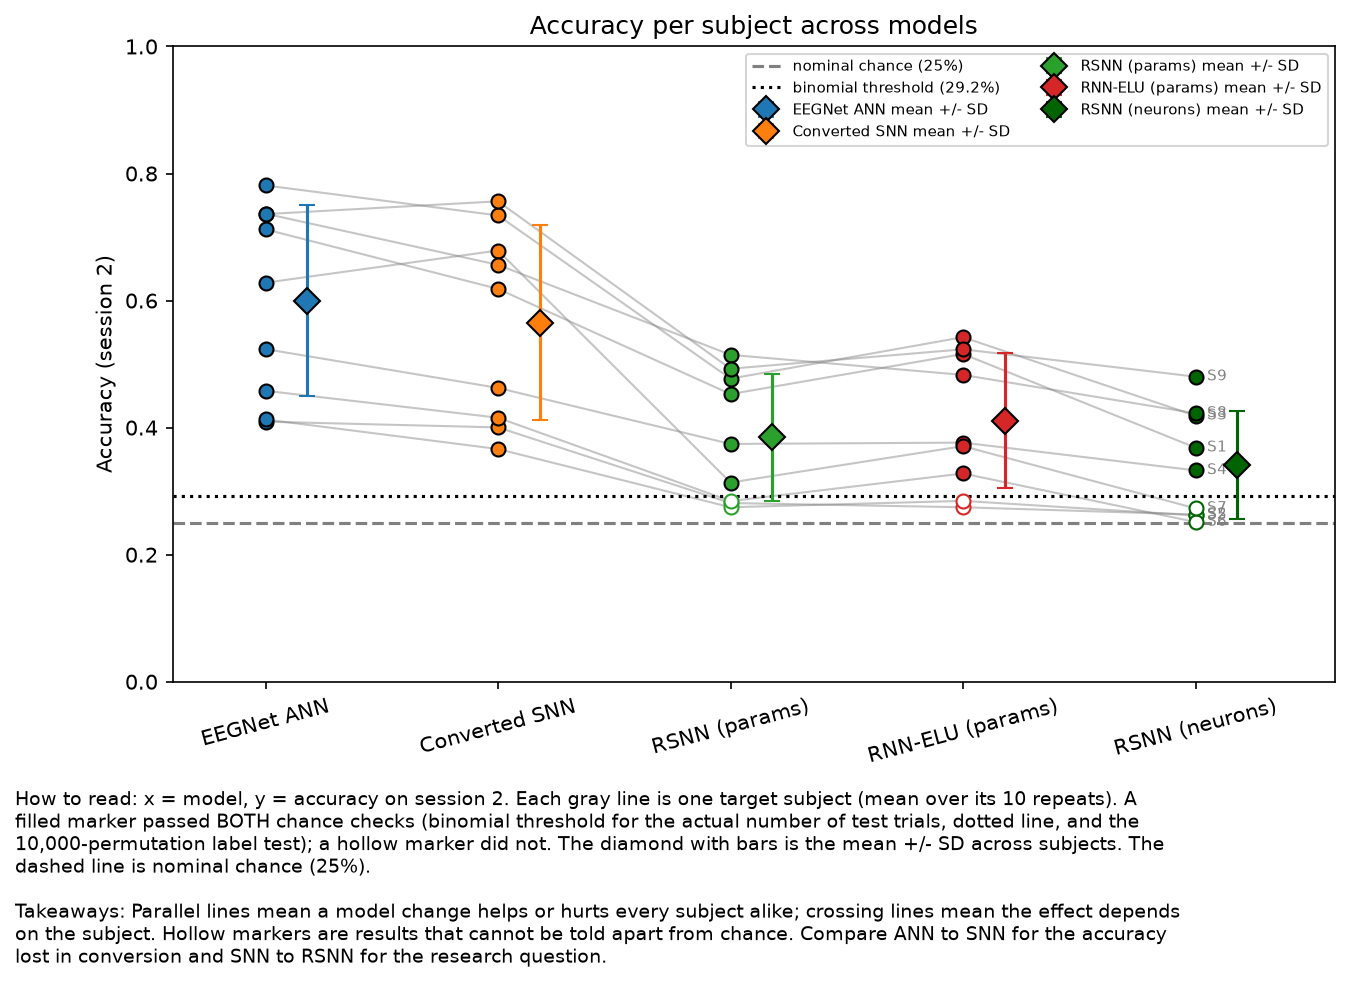
\includegraphics[width=0.75\textwidth, trim=0 99.8bp 0 0, clip]{figures/accuracy_slopes.png}
  \caption{Session-2 accuracy per subject (gray lines, mean over 10 repeats). Filled markers exceeded chance and hollow markers did not. Diamonds show mean $\pm$ SD over subjects. The dotted line is the binomial threshold and the dashed line nominal chance.}
  \label{fig:acc}
\end{figure*}

\subsection{Network size}

Widening the recurrent spiking layer from 17 to 2560 neurons lowered accuracy in all nine subjects, and RSNN-n remained $0.234$ below the SNN (Table~\ref{tab:paired}). Its selected checkpoints came from the first epochs of each phase, at median epoch 6 of 500 in pretraining (89\% of folds by epoch 10) and epoch 4 of 100 in fine-tuning.

\subsection{Training behavior}

The three recurrent configurations trained differently (Fig.~\ref{fig:train}). RSNN-p's median pretraining validation loss stayed between 1.38 and 1.52 throughout ($\ln 4 = 1.386$, median selected epoch 45), and its median training loss was still 1.29 at the end of fine-tuning. RNN-p reached its pretraining validation minimum early (median epoch 12), after which validation loss rose while training loss fell. A loss spike occurred in 17\% of its pretraining folds and 12\% of its fine-tuning folds. RSNN-n's median training loss was lowest at epoch 44 of pretraining and epoch 23 of fine-tuning and then rose, to a maximum of 2.42 and 2.10. The ANN's median pretraining validation loss was lowest at epoch 13 (median selected epoch 17.5), and its fine-tuning validation loss reached its minimum at epoch 99 of 100, with 19\% of folds selecting the final epoch.

\begin{figure*}[!t]
  \centering
  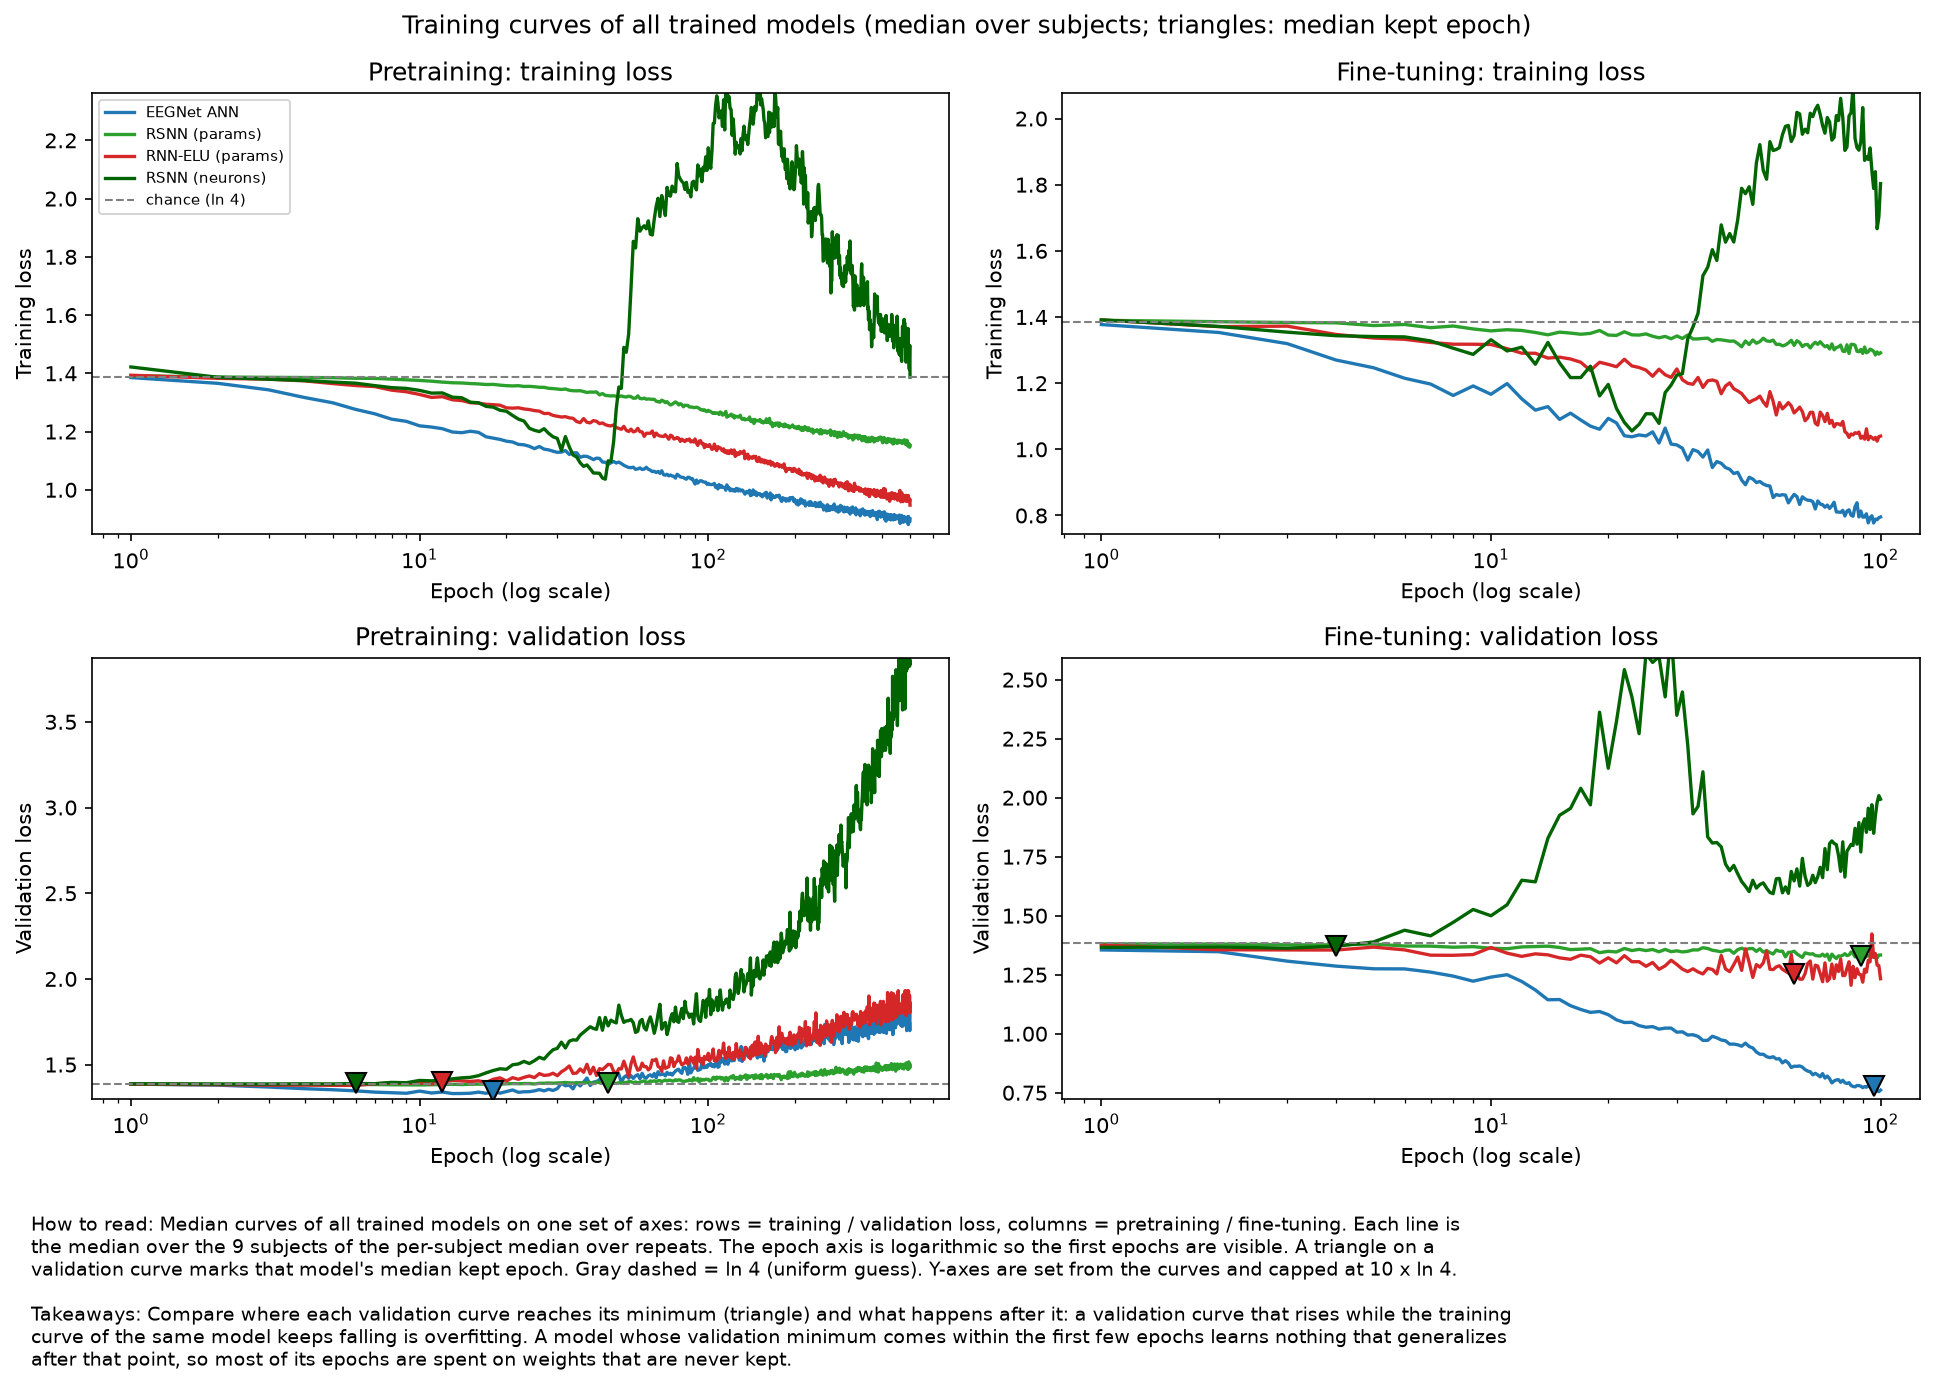
\includegraphics[width=\textwidth, trim=0 94.6bp 0 24.0bp, clip]{figures/training_curves_overlay.png}
  \caption{Median training and validation loss over subjects. Triangles mark the median selected (lowest-validation-loss) epoch. The dashed line is $\ln 4$, the loss of a uniform guess.}
  \label{fig:train}
\end{figure*}

\subsection{Fine-tuning}

Fine-tuning improved every trained model in all nine subjects ($p_\mathrm{Holm} = 0.016$ for each model, Fig.~\ref{fig:ft}). Mean zero-shot accuracy was 0.374 for the ANN and 0.279--0.310 for the recurrent models, and RSNN-p was within 0.06 of chance in seven of nine subjects. Mean gains were 0.225 for the ANN, 0.101 for RSNN-p and RNN-p and 0.062 for RSNN-n, so the RSNN-p deficit to the ANN grew from 0.090 before fine-tuning to 0.215 after it.

\begin{figure}[!t]
  \centering
  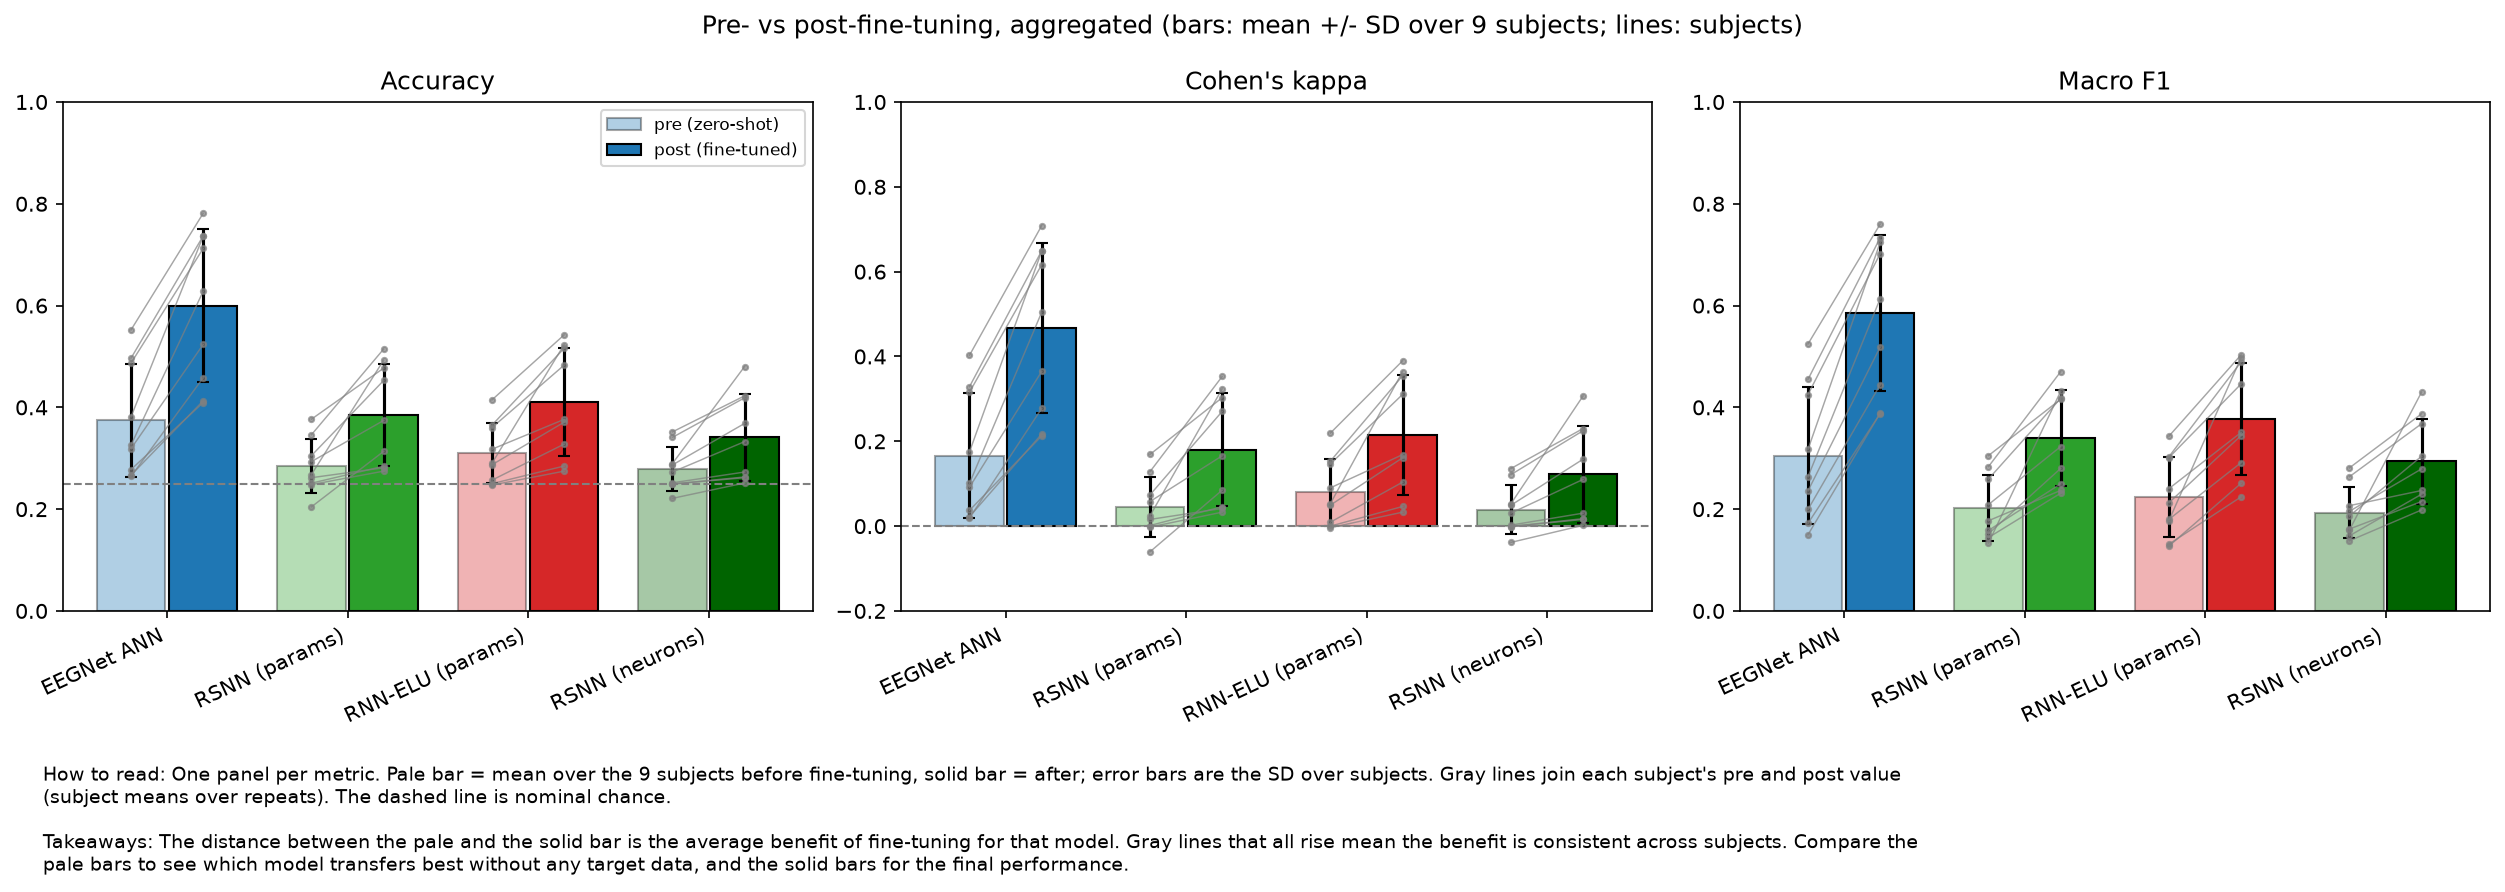
\includegraphics[width=0.9\columnwidth, trim=0 71.5bp 806.3bp 25.9bp, clip]{figures/finetune_pre_post_aggregate.png}
  \caption{Session-2 accuracy of the pretrained model without target data (zero-shot) and after fine-tuning, mean $\pm$ SD over subjects. Gray lines join each subject's values. The dashed line is nominal chance.}
  \label{fig:ft}
\end{figure}

\subsection{Subject differences}

All models ranked the subjects in nearly the same order (Kendall's $W = 0.90$). Subject identity explained 49\% of the variance of the subject-by-model accuracy table, model identity 44\% and their interaction 7\%. S9, S3, S8 and S1 had the highest mean accuracy over models (0.53--0.60) and S5, S2 and S6 the lowest (0.32--0.35). Mean accuracy increased with session-1 class separability ($\rho = 0.87$, $p = 0.002$, session 2: $\rho = 0.90$, $p = 0.001$) and decreased with between-session covariance distance ($\rho = -0.87$, $p = 0.002$) and band-power shift ($\rho = -0.78$, $p = 0.013$). Trial-amplitude variability ($\rho = 0.17$, $p = 0.67$) and artifact rate ($\rho = 0.41$, $p = 0.27$) showed no clear relation. S5 had the lowest separability, S2 the largest between-session change, and S9 the highest separability with the smallest band-power shift.

The recurrent deficit varied in size but never in direction. RSNN-p's accuracy above the 25\% chance level was 43--54\% of the ANN's in S1, S3, S4, S8 and S9, but only 15--20\% in S2, S5, S6 and S7. In S7 the SNN exceeded the ANN in all ten repeats (0.679 vs.\ 0.628), while RSNN-p reached 0.314.

\subsection{Class-specific performance}

Feet was the least accurately classified class for every model (Table~\ref{tab:class}) and was most often confused with tongue, in 28\% of feet trials for the ANN and 40\% for RSNN-p. Pooled ANN recall was higher for left than right hand (0.671 vs.\ 0.621), but right-hand recall was higher in S1, S3, S7 and S8. The SNN predicted left hand for 35.8\% of trials. Tongue had the highest recall of the four classes for every recurrent model, and RSNN-p predicted tongue for 35.2\% of trials, with a tongue precision of 0.408. On hand trials that were predicted as a hand class, RSNN-p chose the correct hand 60\% of the time and the ANN 78\%.

\begin{table}[!t]
  \centering
  \caption{Per-class recall and feet--tongue confusion, pooled over subjects and repeats}
  \label{tab:class}
  \setlength{\tabcolsep}{4pt}
  \begin{tabular}{lcccccc}
    \toprule
    Model & Left & Right & Feet & Tongue & F$\to$T & T pred. \\
    \midrule
    ANN    & 0.671 & 0.621 & 0.467 & 0.640 & 0.275 & 27.3\% \\
    SNN    & 0.729 & 0.637 & 0.398 & 0.498 & 0.167 & 19.3\% \\
    RSNN-p & 0.458 & 0.343 & 0.166 & 0.574 & 0.404 & 35.2\% \\
    RNN-p  & 0.475 & 0.387 & 0.253 & 0.529 & 0.366 & 29.6\% \\
    RSNN-n & 0.378 & 0.296 & 0.225 & 0.467 & 0.351 & 31.1\% \\
    \bottomrule
  \end{tabular}
  \\[2pt]
  \footnotesize F$\to$T is the share of feet trials predicted as tongue. T pred.\ is the share of all predictions that were tongue (25\% of trials are tongue).
\end{table}

\section{Discussion}

\subsection{Answer to the research question}

Under subject-level, cross-session evaluation, neither RSNN decoded as accurately as EEGNet. RSNN-p was less accurate than EEGNet and its converted SNN in every subject and by every metric, and RSNN-n was less accurate still. The results therefore do not support the hypothesis that a single recurrent spiking layer, trained under these conditions, can replace EEGNet's dedicated temporal, spatial and feature-summarizing layers. However, they also do not show that it cannot. RSNN-p exceeded chance in six of nine subjects and RSNN-n in five, so a single recurrent layer did extract class information from multichannel EEG with no dedicated spatial or temporal filters. Every setting used to train it, including the learning rate, dropout, batch size and number of epochs, was chosen for EEGNet, a feedforward convolutional network, and the recurrent models probably needed different settings (Section~\ref{sec:trainability}). The evidence comes from one recurrent design tested at two sizes. Whether better-suited training, a different recurrent design or the additions proposed in Section~\ref{sec:future} would close the gap requires further research.

\subsection{Spiking is not the main source of the deficit}

The two spiking comparisons locate most of the deficit. Converting EEGNet to an SNN cost about 0.05 in accuracy, and replacing the LIF neurons of RSNN-p with ELU units changed accuracy by about 0.03. Neither difference was significant. With nine subjects this does not show that spiking has no cost, but the upper ends of the two confidence intervals (0.081 and 0.063) lie well below the cost of about 0.2 of replacing EEGNet's layers with one recurrent layer without spiking (RNN-p), which was consistent across all nine subjects. The small conversion cost agrees with reports that a converted EEGNet performs comparably to its ANN \cite{chen2026} and that SNNs are generally somewhat less accurate than comparable CNNs \cite{zhang2025}. The deficit therefore lies mainly in how the recurrent models extract spatial and temporal features, not in spiking.

\subsection{Spatial extraction}

EEGNet-4,2 learns two spatial filters for each of its four frequency filters. The recurrent models instead combine the 22 channels in one linear projection onto the recurrent layer at every step, before any temporal processing. Three results suggest that this spatial pathway accounts for much of the gap.
\begin{itemize}
  \item The recurrent models lost most on the left/right hand distinction, which depends on a lateralized spatial pattern (Fig.~\ref{fig:topo}). On hand trials predicted as a hand class, RSNN-p chose the correct hand less often than the ANN (60\% vs.\ 78\%).
  \item The recurrent models' relatively high tongue recall partly reflects a bias toward predicting tongue. Tongue imagery produced the broadest, least lateralized band-power change, which a model without spatial filters may detect more easily than lateralized hand patterns.
  \item On trials the ANN missed, the recurrent models were correct only 26\% of the time. They did not capture information that the convolutional model lacked.
\end{itemize}

\subsection{Temporal extraction and memory}

The recurrent models also had to extract temporal features differently. Each EEGNet convolution sees a window of samples at once. The RSNNs see one sample per step, so information from earlier in the trial must be carried forward in their state. Their membrane memory is short. With $\beta = 0.9$ at 128~Hz, an input's contribution to the membrane potential falls to $1/e$ of its initial value after about 74~ms (9--10 steps), less than one cycle of the mu rhythm (77--125~ms), while each trial lasts 2~s. Longer memory must therefore come from the recurrent weights, and in this design every recurrent connection passes activity on after exactly one step. A plausible hypothesis is that, without a mechanism for delaying signals between neurons, the RSNNs lacked the effective memory needed to integrate the band-power changes that distinguish the classes over the trial. This hypothesis was not tested. It is consistent with RSNN-p's validation loss remaining near $\ln 4$ throughout pretraining and with RSNN-n not performing better, but both results have other possible explanations, including the training settings discussed below. The input encoding may also matter. RSNNs have outperformed feedforward SNNs on speech, gesture and cortical spike-train data \cite{yin2021,liu2025,liu2024}, whose inputs are already event streams, whereas continuous EEG had to be injected as a current one sample at a time. Whether a longer time constant or a learned encoding would change the result was not tested.

The study also cannot say whether inter-recurrence added anything to intra-recurrence. No model was trained that differs from RSNN-p only by lacking connections between neurons, so whether the trained inter-recurrence helped, hurt or made no difference within this design is unknown.

\subsection{Network size and trainability}
\label{sec:trainability}

The size comparison does not show that capacity is irrelevant. RSNN-n's selected checkpoints came from the first few epochs, and its training loss later rose. Under the shared settings, the wider recurrent model was therefore not trained to convergence, so the comparison mixes capacity with optimization. What the results do show is that parameter count alone was not the limiting factor, because EEGNet with 796 parameters outperformed RSNN-n with 6.6 million.

Each recurrent configuration failed in a different way. RSNN-p underfit, RNN-p overfit early with loss spikes, and RSNN-n became unstable. This is the main alternative explanation for the recurrent deficit. The learning rate, schedule, batch size and dropout were chosen for a convolutional ANN. Keeping them fixed made the comparison controlled but probably disadvantaged the recurrent models. How much tuning would narrow the gap is unknown. RSNN-p's high final training loss shows that it was not at its capacity.

\subsection{Transfer, fine-tuning and implications for users}

Zero-shot accuracy was low for every model. The ANN's 0.374 is close to the cross-subject accuracy near 40\% that the EEGNet authors reported without target-subject data \cite{lawhern2018}. Most of each model's final accuracy came from 230 session-1 trials of the target subject. For people who would use a motor imagery BCI to control a mobility device, this means that under this paradigm a subject-specific calibration session remains necessary. Data from other users was not enough.

Whether pretraining improves the final accuracy at all remains open, because no model was fine-tuned from random initialization. The recurrent models gained less from fine-tuning than the ANN, so their deficit is partly a deficit in adapting to a new user. One implementation difference may contribute and is untested. The recurrent models normalized their inputs with statistics fixed from the pretraining subjects, whereas the ANN's batch-normalization statistics updated during fine-tuning and the SNN was calibrated on target-subject data.

\subsection{Subject and class differences}

Subject identity explained about as much variance as model choice (49\% vs.\ 44\%), and every model ranked the subjects almost identically. Subjects with weaker class separability and larger between-session change were harder for every model. These are correlations across nine subjects, consistent with weaker or less stable motor imagery patterns in some recordings rather than with a property of any one decoder. A mean over subjects therefore hides users who are poorly served by every decoder tested. This supports reporting at the subject level rather than over non-independent folds \cite{lawhern2018}. Because small differences can arise from random fluctuation \cite{tangermann2012}, only effects that were consistent across subjects are interpreted here.

The recurrent deficit was proportionally largest in middle- and low-accuracy subjects (S2, S5, S6, S7). This suggests that the recurrent models captured mainly the strongest class information in each recording. S7 stands out, because both convolutional models decoded it well but the recurrent models did not. Why is unresolved.

Feet was the hardest class for every model. In the class topographies it produced the smallest band-power deviation from the all-class mean. Feet and tongue imagery both tend to enhance rather than suppress the mu rhythm over the hand areas \cite{pfurtscheller2006}, and both are bilateral, so the left/right contrast that separates the hand classes cannot separate them. The pooled left-hand advantage was not consistent across subjects. The SNN's left-hand bias arose during conversion, not in the data. The dataset reports no handedness, so handedness effects could not be examined.

\subsection{Limitations and future work}
\label{sec:future}

\begin{itemize}
  \item \textbf{Shared hyperparameters.} The recurrent models used settings chosen for EEGNet.
  \item \textbf{Missing controls.} No model with the RSNN's topology was trained with only intra-recurrence or without recurrence, and network size was tested at only two points, one of which did not train stably.
  \item \textbf{Input normalization.} It differed between the recurrent and convolutional models.
  \item \textbf{Efficiency not measured.} Energy, latency and spike counts were not measured, so the low-power motivation for SNNs was not tested.
  \item \textbf{Fixed scope.} All models used one 0.5--2.5~s window from one dataset and were evaluated offline, so performance with other windows, other datasets or in online closed-loop use is unknown.
  \item \textbf{Sample.} Nine subjects from one laboratory, recorded with a cue-based offline paradigm, are a small and narrow sample that does not represent users with complex mobility needs. Each subject's session 1 also contributes to the pretraining of the other subjects' models, so the nine cases are only approximately independent.
\end{itemize}

The most direct next step is to separate the two kinds of recurrence within the existing design. Evaluating the saved RSNN-p checkpoints with the connections between neurons set to zero, while keeping each neuron's self-connection, would show without retraining whether inter-recurrence contributes. Setting all recurrent weights to zero would leave only the membrane. A feedforward LIF control with the same input projection and readout, trained from scratch, would separate recurrence from the spatial pathway.

A second direction addresses the memory hypothesis. The conventional way to lengthen memory in a recurrent network is to use gated units such as LSTM units or GRUs \cite{hochreiter1997,cho2014}, which learn when to keep or overwrite their state and have already been used inside a spiking EEG decoder \cite{gong2023}. Gating adds memory but not delays, and it moves the model away from biological neurons. A more biologically motivated option is to give connections a trainable transmission delay, analogous to the conduction delay set by an axon's myelination, which is itself regulated by neural activity in the brain \cite{fields2015}. This idea has been explored outside EEG. Trainable delays improved feedforward SNNs on spoken-word and speech-command benchmarks \cite{sun2023,hammouamri2024}, and in one study fixed random delays helped while learned delays helped more \cite{hammouamri2024}. DelRec learned delays in the recurrent connections of an RSNN, motivated explicitly by myelination. It improved on a delay-free RSNN in time-series forecasting, localization and activity-recognition tasks and reported state-of-the-art accuracy on a spiking speech-command benchmark \cite{queant2025}. Delays have also been adjusted by myelination-inspired learning rules rather than by gradient descent \cite{hazan2022,nadafian2024}. To the best of our knowledge, learnable delays have not been evaluated in an RSNN for motor imagery EEG decoding.

Such a test should keep the present protocol so that any gain can be attributed to the delays, with the same cross-session split, subject-level statistics and approximate parameter matching. One delay per neuron (an axonal delay) adds only $H$ parameters, 17 for RSNN-p, whereas one delay per connection (a synaptic delay) adds one per recurrent connection, so the two should be compared at matched size. The delayed RSNN should be compared with the same network with zero delays and with fixed random delays, to separate the effect of learning delays from that of simply having them, and with a gated recurrent baseline. The longest allowed delay should span several cycles of the mu and beta rhythms. Because delayed spikes must be buffered, the memory and computational cost of delays on embedded or neuromorphic hardware should be reported alongside accuracy \cite{patinosaucedo2023}.

Finally, the RSNNs were evaluated with a single set of hyperparameters, most of them taken from EEGNet or chosen once. A systematic study of the RSNN's hyperparameters, each tuned on pretraining-validation data only, would show how much of the gap reflects the design and how much reflects the settings it was given, and which choices matter most for EEG decoding.

\section{Conclusion}
\label{sec:conclusion}

Under subject-level, cross-session evaluation on BCI Competition IV dataset 2a, neither of two RSNNs that extract spatial and temporal features within one recurrent spiking layer decoded four-class motor imagery as accurately as EEGNet, which uses dedicated temporal, spatial and feature-summarizing layers. The 17-neuron RSNN was less accurate than EEGNet in every subject (median paired difference in accuracy $-0.222$) and exceeded chance in six of nine subjects, and the 2560-neuron RSNN was less accurate still, whereas EEGNet and its converted SNN exceeded chance in all nine. The effect of spiking was small and not significant in either the feedforward or the recurrent design, so most of the deficit lies in replacing EEGNet's dedicated layers with one recurrent layer. The main contribution of this study is a subject-level, cross-session comparison with spiking and non-spiking controls, which shows that under shared training settings the recurrent design, not spiking, accounts for most of the accuracy gap.

The recurrent models were weakest on the lateralized left/right hand distinction, which points to their single linear spatial projection. Their temporal extraction may also have been limited by little effective memory over a 2~s trial. Neither explanation was tested directly, and the study did not separate intra- from inter-recurrence. Because both RSNNs still exceeded chance in most subjects and were trained with settings chosen for EEGNet, the results do not rule out that a recurrent spiking layer can replace dedicated filters. Useful next steps are to isolate inter-recurrence in the existing model, to add learnable transmission delays to the recurrent connections and test them against delay-free and fixed-delay versions under the same protocol, and to study the RSNN's hyperparameters systematically.

\section*{Data and Code Availability}

BCI Competition IV dataset 2a is openly available from the BCI Competition IV website \cite{brunner2008} and through MOABB as BNCI2014\_001 \cite{jayaram2018,moabbdoc2014001}. The recordings are not redistributed with this work. The analysis code is available at \url{https://github.com/thesixtium/bmen-600-group-11}, and the results reported here were produced with its most recent version. The repository README describes how to obtain the data, set up the software environment, run the training and analysis pipelines, and identify the scripts that produce the reported figures and tables.

\section*{AI-Assisted Work}

Claude (Anthropic) and Microsoft Copilot were used as supporting tools to generate and revise analysis code and to edit the text of this paper for clarity. Claude was also used to check the bibliography against publisher and index records, and it suggested two references \cite{pfurtscheller2006,luo2018}, which the authors checked against the original papers. No AI tool labeled, transformed or analyzed the data directly. All data processing was performed by the project code. The authors reviewed all AI-generated code in full and tested the pipeline with short smoke-test runs before the full experiments. The reported methods, statistics, tables and figures were checked against the implementation and the saved results, and all AI-assisted text was reviewed and revised by the authors. The authors take full responsibility for the research and the content of this paper.

\section*{Author Contributions}

% Template: replace each placeholder with an author's name and list that author's contributions.
% Suggested categories: research question, literature review, data preparation, analysis, code,
% figures, interpretation, writing, revision. Add or remove rows as needed.
\begin{itemize}
  \item \textbf{[Author 1]:} [contributions]
  \item \textbf{[Author 2]:} [contributions]
  \item \textbf{[Author 3]:} [contributions]
\end{itemize}

\bibliographystyle{IEEEtran}
\bibliography{references}

\end{document}